\documentclass[twocolumn,10pt]{article}

\usepackage{authblk}
\usepackage{bera}
\usepackage[utf8]{inputenc}
\usepackage{graphicx}
\usepackage{booktabs}
\usepackage{hyperref}
\usepackage{acronym}

% TITLE
\title{Medical Specialty Classification from Clinical Notes: Does a Language Model Beat Classical Text Features?}


% AUTHORS
\author{Group 26 | André Maçorano (110203, 25\%), David Fonseca (109494, 25\%), Miguel Ferreira (110268, 25\%), Vasyl Podvirnyy (109545, 25\%)}
%\affil{Instituto Superior Técnico, Universidade de Lisboa}

\begin{document}

\maketitle

% ============================================================
\section{Introduction}
% ============================================================

Automatically routing clinical documents to the correct medical specialty has clear practical value for hospital administration and electronic health record management. Yet clinical notes are short, noisy, and written in highly specialised language, which makes the task non-trivial.

In this work we ask: does a domain-specific language model, fine-tuned on short clinical descriptions, outperform a classical classifier trained on the full available text? Our experiments use a dataset of 2{,}613 annotated records across 12 specialties, heavily imbalanced towards Surgery, and we track both accuracy and per-class F1 score to account for that imbalance.

% Acronym definitions (used consistently throughout)
\acrodef{nlp}{Natural Language Processing}
\acrodef{tfidf}{Term Frequency--Inverse Document Frequency}
\acrodef{mnb}{Multinomial Naive Bayes}
\acrodef{lr}{Logistic Regression}
\acrodef{svm}{Support Vector Machine}
\acrodef{eda}{Easy Data Augmentation}


% ============================================================
\section{Data}
% ============================================================

\subsection{Data Analysis}

The base dataset provided for this project consists of 2{,}613 annotated clinical records distributed across 12 medical specialties. Each record contains five fields: \texttt{medical\_specialty} (the target label to predict), \texttt{description} (a short one-to-two sentence summary of the visit), \texttt{sample\_name} (the procedure or visit type), \texttt{transcription} (the full clinical note), and \texttt{keywords} (a comma-separated list of relevant terms).

\textbf{Class distribution.} Table~\ref{tab:class_dist} shows the distribution of samples across the 12 specialties. The dataset exhibits severe class imbalance: the majority class (Surgery) contains 876 samples, whereas the minority class (Dermatology) contains only 25 samples --- a ratio of approximately 35:1. Such imbalance is known to cause classifiers to default to frequent classes, resulting in near-zero recall for minority classes \cite{imbalance_survey}.

\begin{table}[h]
\centering
\caption{Class distribution of the training set.}
\label{tab:class_dist}
\small
\begin{tabular}{lrr}
\toprule
\textbf{Specialty} & \textbf{Count} & \textbf{\%} \\
\midrule
Surgery                  & 876 & 33.5\% \\
Cardiovascular-Pulmonary & 299 & 11.4\% \\
Orthopedic               & 292 & 11.2\% \\
Radiology                & 217 &  8.3\% \\
General Medicine         & 207 &  7.9\% \\
Gastroenterology         & 192 &  7.3\% \\
Neurology                & 181 &  6.9\% \\
Obstetrics-Gynecology    & 135 &  5.2\% \\
Neurosurgery             &  78 &  3.0\% \\
Ophthalmology            &  71 &  2.7\% \\
Psychiatry-Psychology    &  40 &  1.5\% \\
Dermatology              &  25 &  1.0\% \\
\bottomrule
\end{tabular}
\end{table}

Figure~\ref{fig:class_dist} provides a visual representation of this distribution. Figure~\ref{fig:text_lengths} in the Appendix shows the average word count per field and specialty.

\begin{figure}[h]
\centering
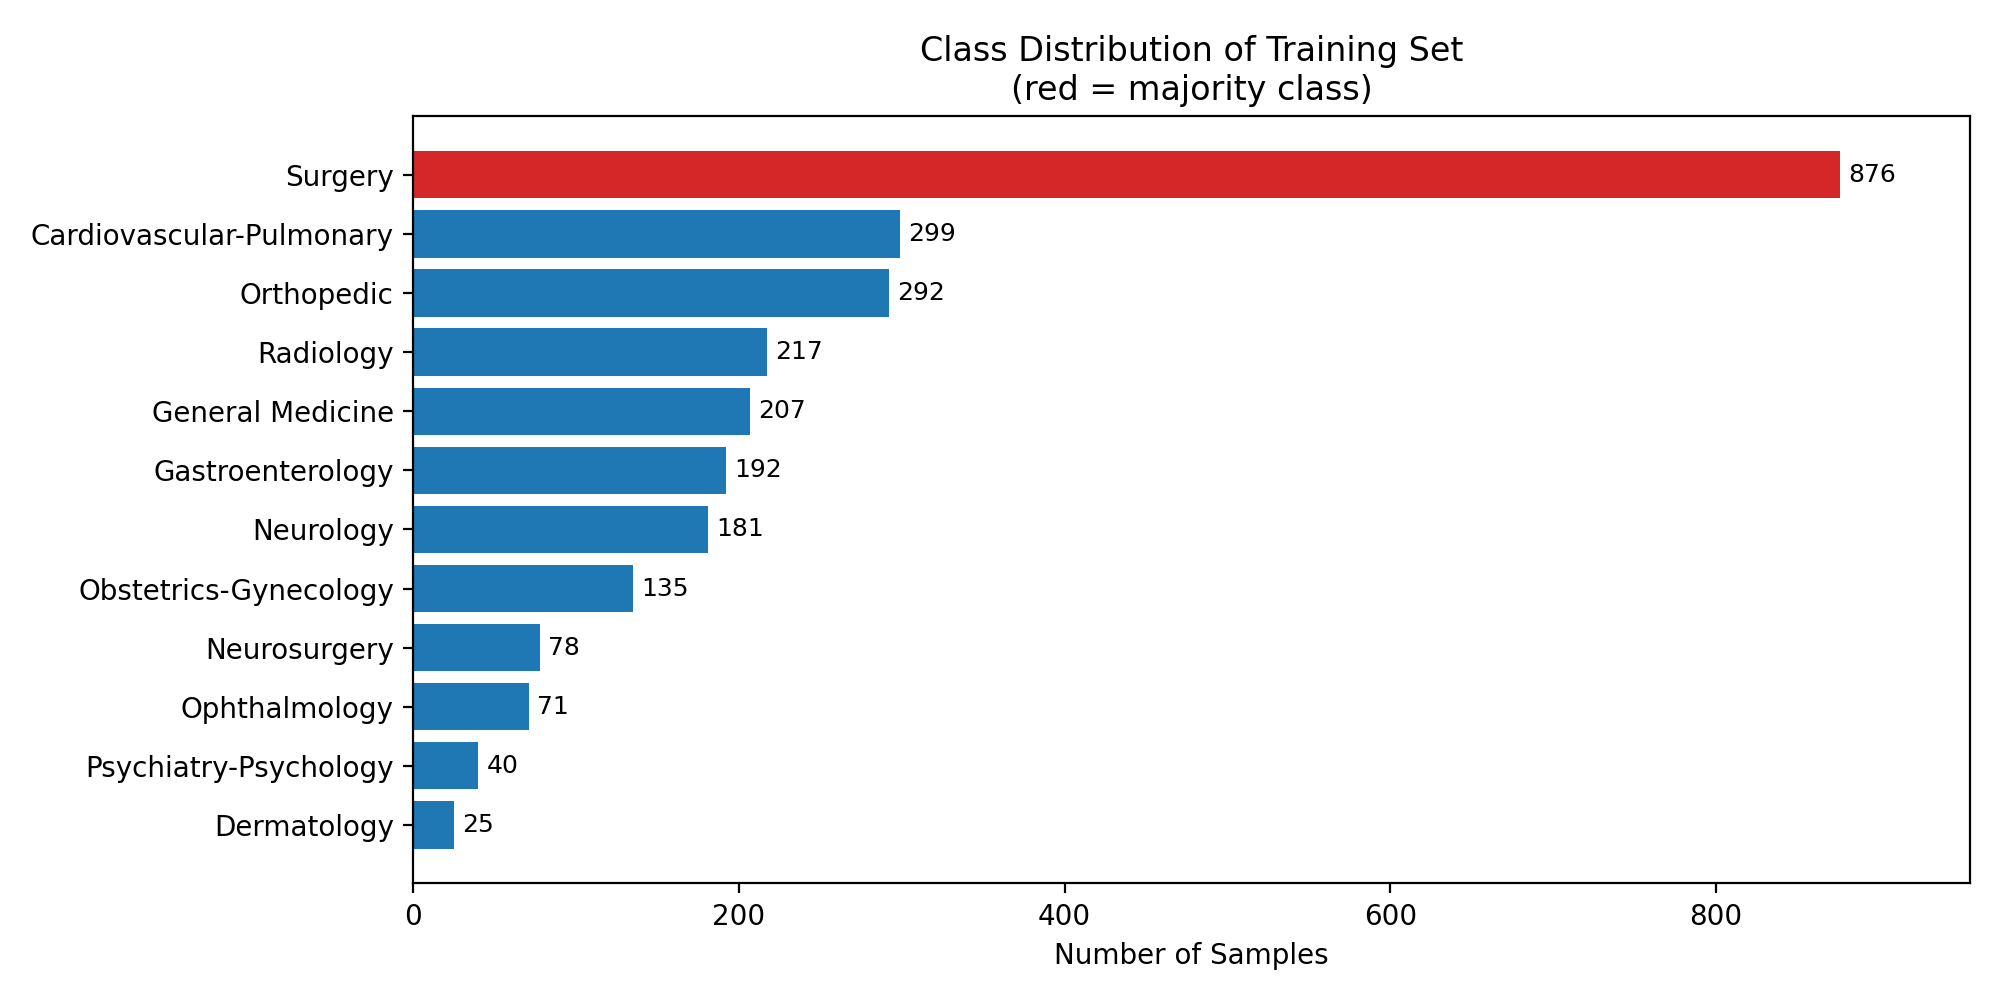
\includegraphics[width=\linewidth]{figures/fig1_class_distribution.png}
\caption{Class distribution of the base dataset. Surgery dominates with 33.5\% of all records.}
\label{fig:class_dist}
\end{figure}

\textbf{Observation 1 --- Field length varies substantially across specialties.} The \texttt{description} field is short and consistent (mean: 28.4 words), making it suitable for models with strict token limits. The \texttt{transcription} field is significantly longer (mean: 452.2) with high variance: Radiology averages 275.8 words, whereas Psychiatry-Psychology averages 823.7. A classical model trained on the full transcription may introduce a length bias favouring verbose specialties.

\textbf{Observation 2 --- Vocabulary overlap introduces classification ambiguity.} Frequent terms in the \texttt{description} field reveal significant lexical overlap between Surgery and Neurosurgery (shared top terms: \emph{right}, \emph{left}, \emph{patient}), making separation difficult without specialty-specific terms (e.g., \emph{discectomy}). In contrast, Radiology contains highly distinctive vocabulary (\emph{MRI}, \emph{ultrasound}) making it easier to identify. Finally, 30 empty transcriptions and 158 short descriptions (under 5 words) were found, representing potential noise.

\subsection{Data Augmentation}

The class imbalance identified in Section~2.1 motivates an explicit data augmentation strategy. An unbalanced and relatively small dataset is a poor training base: without intervention, a classifier defaults to predicting the majority class (Surgery), resulting in near-zero recall for underrepresented specialties. To build a more balanced training set, we applied programmatic data augmentation to all 11 minority classes that had fewer than 400 samples, generating numerous new records to reach a more uniform distribution.

\textbf{Augmentation techniques.} To ensure diversity without losing clinical meaning, we implemented 15 text transformation variants inspired by the \ac{eda} framework~\cite{wei2019eda}. These include beneficial techniques such as curated clinical synonym replacement (e.g., \emph{patient} $\rightarrow$ \emph{individual}), structural changes (e.g., sentence deletion, abbreviation expansion, and filler-word compression), and surface variations (e.g., case and punctuation changes). Additionally, intentional noise (random deletion and word swaps) was introduced as a controlled ablation. 

Crucially, all protected medical terminology (abbreviations, dosages, and hyphenated compounds) was shielded from modification using a rule-based filter to preserve clinical precision. 

The final augmented training set contains 5{,}624 records. Class distribution after augmentation is shown in Table~\ref{tab:aug_dist}.

\begin{table}[h]
\centering
\caption{Class distribution before and after augmentation.}
\label{tab:aug_dist}
\small
\begin{tabular}{lrr}
\toprule
\textbf{Specialty} & \textbf{Before} & \textbf{After} \\
\midrule
Surgery                  & 876 & 876 \\
Cardiovascular-Pulmonary & 299 & 460 \\
Orthopedic               & 292 & 459 \\
Radiology                & 217 & 444 \\
General Medicine         & 207 & 442 \\
Gastroenterology         & 192 & 438 \\
Neurology                & 181 & 436 \\
Obstetrics-Gynecology    & 135 & 427 \\
Neurosurgery             &  78 & 415 \\
Ophthalmology            &  71 & 414 \\
Psychiatry-Psychology    &  40 & 408 \\
Dermatology              &  25 & 405 \\
\midrule
\textbf{Total}           & \textbf{2,613} & \textbf{5,624} \\
\bottomrule
\end{tabular}
\end{table}

% ============================================================
\section{Models}
% ============================================================
% TODO: To be completed after Phase 3.

% ============================================================
\section{Experimental Setup}
% ============================================================
% TODO: To be completed after Phase 3.

\subsection{Parameters/Hyperparameters}
% TODO: To be completed after Phase 3.

% ============================================================
\section{Results}
% ============================================================
% TODO: To be completed after Phase 3--4.

% ============================================================
\section{Discussion}
% ============================================================
% TODO: To be completed after Phase 4 (requires misclassified examples).

% ============================================================
\section{Future Work}
% ============================================================
% TODO: To be completed last.

% ============================================================
\section*{Bibliography}
% ============================================================

\bibliographystyle{apalike}
\bibliography{biblio}

% One page at most. Only the first two pages of the paper will be read. The appendix should only contain complementary information.

\appendix

\section*{Appendix A: Extra Figures and Tables}

\begin{figure}[h]
\centering
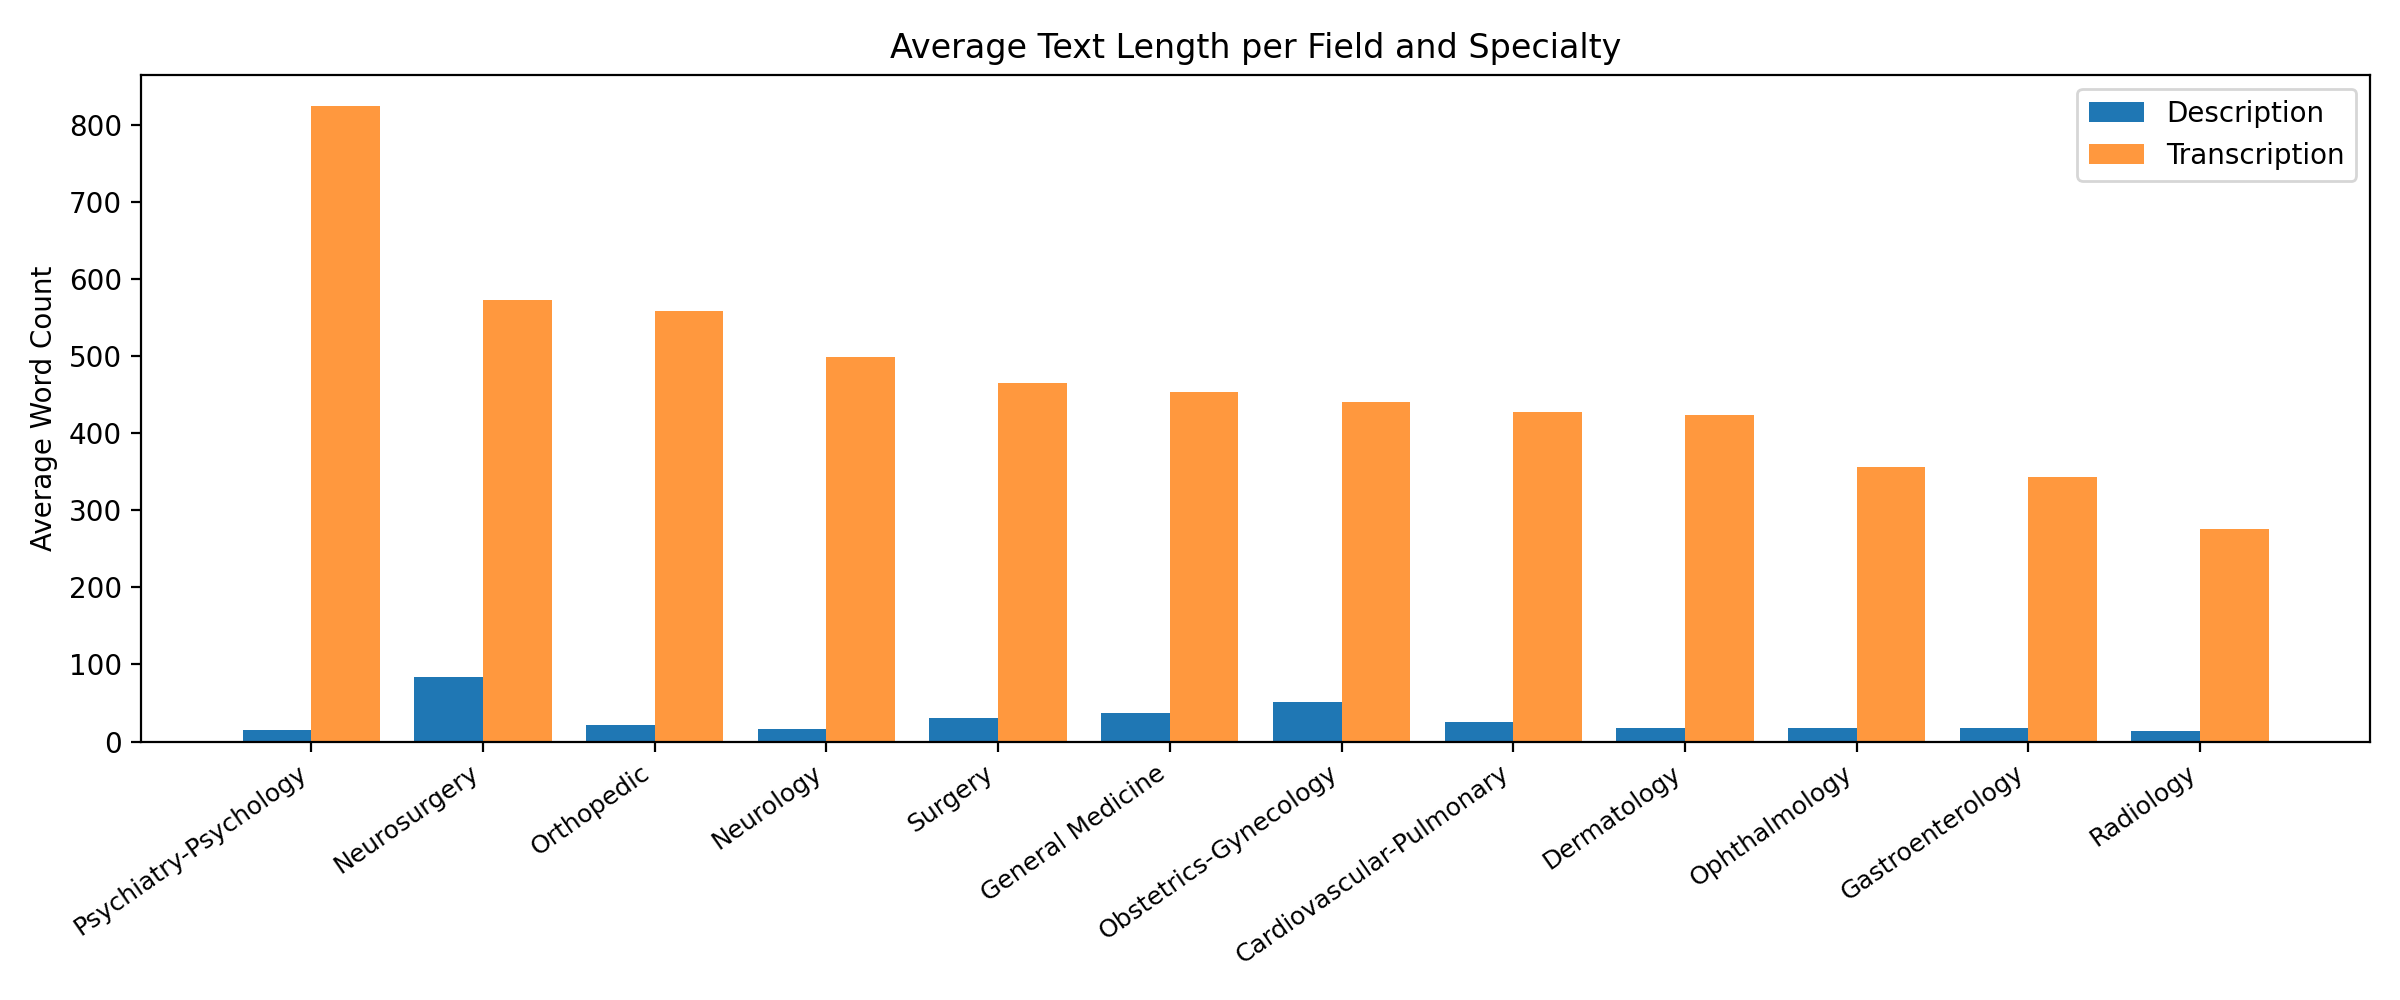
\includegraphics[width=\linewidth]{figures/fig2_text_lengths.png}
\caption{Average word count per field (description vs.\ transcription) across all 12 specialties.}
\label{fig:text_lengths}
\end{figure}






\end{document}
